% SDRTerm — FM broadcast demodulation pipeline walkthrough
%
% Build with:  pdflatex pipeline.tex   (twice, so ToC + refs resolve)

\documentclass[11pt,a4paper]{article}

\usepackage[margin=2cm]{geometry}
\usepackage{amsmath,amssymb,amsthm}
\usepackage{tikz}
\usepackage{pgfplots}
\pgfplotsset{compat=1.18}
\usetikzlibrary{arrows.meta, positioning, shapes.geometric, calc,
                decorations.pathreplacing, backgrounds, fit, patterns}
\usepackage{listings}
\usepackage{xcolor}
\usepackage{hyperref}
\usepackage{caption}
\usepackage{booktabs}
\usepackage{siunitx}
\usepackage{parskip}

\hypersetup{
  colorlinks=true,
  linkcolor=blue!70!black,
  urlcolor=blue!60!black,
  citecolor=black,
}

\lstset{
  basicstyle=\ttfamily\small,
  frame=single,
  breaklines=true,
  showstringspaces=false,
  columns=fullflexible,
  keepspaces=true,
  backgroundcolor=\color{gray!5},
}

\title{Wideband FM Demodulation\\
       \large A Walkthrough of SDRTerm's \texttt{fm} Plugin\\
       (Written for a Dumb Monkey Who Just Wants Radio)}
\author{SDRTerm project}
\date{\today}

\begin{document}
\maketitle
\tableofcontents
\vspace{2em}

%═══════════════════════════════════════════════════════════════════
\section{Introduction}
%═══════════════════════════════════════════════════════════════════

FM broadcast radio (the 88--108\,MHz band you tune your car stereo to)
is \emph{wideband} FM: each station occupies about \SI{200}{kHz} and
carries a frequency deviation of \(\pm\SI{75}{kHz}\) around its carrier.
The audio you eventually hear is buried in the \emph{instantaneous
frequency} of that carrier -- deviate up when the audio waveform swings
positive, deviate down when it swings negative.

The plugin turns a stream of complex IQ samples off the SDR into a
stream of 48\,kHz audio samples the operating system's audio stack can
play.  Nine stages, in this order:

\begin{center}
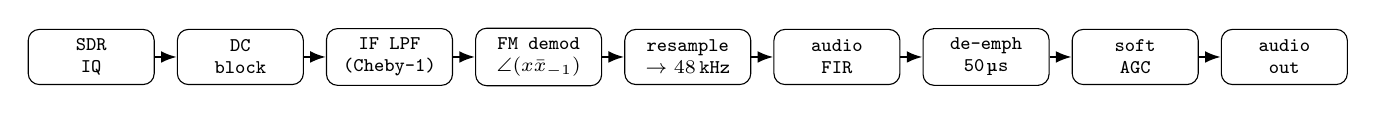
\begin{tikzpicture}[node distance=0.28cm,
  block/.style={draw, rounded corners, minimum width=1.6cm, minimum height=0.7cm,
                align=center, font=\scriptsize\ttfamily},
  arrow/.style={-{Latex[length=2mm]}, thick}]

  \node[block] (sdr)                 {SDR\\IQ};
  \node[block, right=of sdr]  (dc)   {DC\\block};
  \node[block, right=of dc]   (if)   {IF LPF\\(Cheby-1)};
  \node[block, right=of if]   (dem)  {FM demod\\$\angle(x\bar x_{-1})$};
  \node[block, right=of dem]  (rs)   {resample\\$\to 48$\,kHz};
  \node[block, right=of rs]   (alpf) {audio\\FIR};
  \node[block, right=of alpf] (de)   {de-emph\\50\,µs};
  \node[block, right=of de]   (agc)  {soft\\AGC};
  \node[block, right=of agc]  (out)  {audio\\out};

  \draw[arrow] (sdr)  -- (dc);
  \draw[arrow] (dc)   -- (if);
  \draw[arrow] (if)   -- (dem);
  \draw[arrow] (dem)  -- (rs);
  \draw[arrow] (rs)   -- (alpf);
  \draw[arrow] (alpf) -- (de);
  \draw[arrow] (de)   -- (agc);
  \draw[arrow] (agc)  -- (out);
\end{tikzpicture}
\end{center}

Each block below gets its own section, with the maths and a picture.

%═══════════════════════════════════════════════════════════════════
\section{The Signal We're Trying to Decode}
%═══════════════════════════════════════════════════════════════════

\subsection{What a broadcast FM station actually transmits}

The RF signal on \(f_c\) (say, \(f_c = \SI{105.8}{MHz}\)) is
\begin{equation}
s_{\mathrm{RF}}(t) \;=\; A\,\cos\!\Big(2\pi f_c t \;+\;
    2\pi\,k_f\!\!\int_{-\infty}^{t}\!\!m(\tau)\,d\tau\Big),
\end{equation}
where \(m(t)\) is the \emph{modulating signal} -- for a mono station,
just the audio waveform; for a stereo station, a more elaborate MPX
(multiplex) baseband we describe next.  The \emph{frequency-deviation
constant} \(k_f\) is chosen so that the peak deviation is \SI{75}{kHz}.

\subsection{The stereo MPX baseband}

Modern FM stations transmit an audio baseband that isn't just plain
audio -- it's a multiplex of several signals stacked in frequency:

\begin{center}
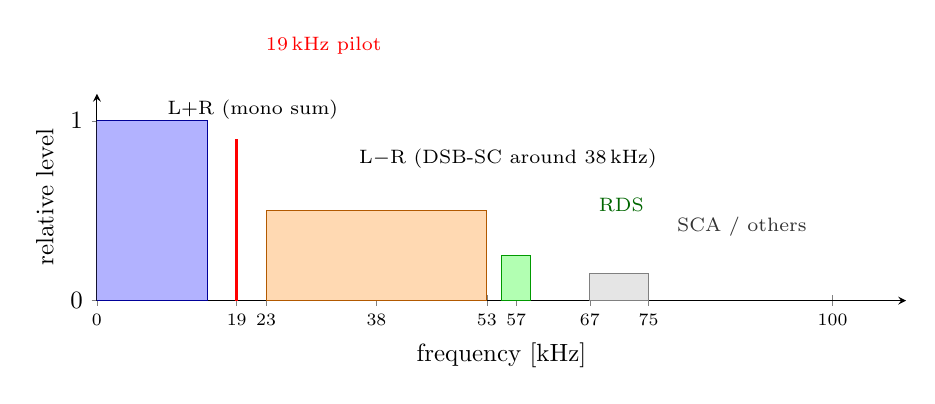
\begin{tikzpicture}[scale=0.90]
  \begin{axis}[width=13cm, height=4.5cm,
    ymin=0, ymax=1.15,
    xlabel={frequency [\si{kHz}]}, ylabel={relative level},
    axis y line=left, axis x line=bottom,
    xmin=0, xmax=110, xtick={0,19,23,38,53,57,67,75,100},
    xticklabel style={font=\scriptsize},
    ytick={0,1}]
    % L+R sum, 30 Hz – 15 kHz
    \addplot[fill=blue!30, draw=blue!60!black] coordinates {(0,0)(0,1)(15,1)(15,0)} \closedcycle;
    % 19 kHz pilot
    \addplot[very thick, red] coordinates {(19,0)(19,0.9)};
    % L-R DSB-SC at 38 kHz, ±15 kHz
    \addplot[fill=orange!30, draw=orange!70!black] coordinates {(23,0)(23,0.5)(53,0.5)(53,0)} \closedcycle;
    % RDS at 57 kHz, ±2 kHz
    \addplot[fill=green!30, draw=green!60!black] coordinates {(55,0)(55,0.25)(59,0.25)(59,0)} \closedcycle;
    % SCA / DirectBand at 67/92
    \addplot[fill=gray!20, draw=gray] coordinates {(67,0)(67,0.15)(75,0.15)(75,0)} \closedcycle;
  \end{axis}
  \node[font=\scriptsize] at (2.2, 2.7) {L+R (mono sum)};
  \node[font=\scriptsize, red] at (3.2, 3.6) {19\,kHz pilot};
  \node[font=\scriptsize] at (5.8, 2.0) {L$-$R (DSB-SC around 38\,kHz)};
  \node[font=\scriptsize, green!40!black] at (7.4, 1.35) {RDS};
  \node[font=\scriptsize, gray!40!black] at (9.1, 1.05) {SCA / others};
\end{tikzpicture}
\end{center}

For a plain mono demodulator like ours, only the L+R band matters: the
\emph{audio LPF} at 15\,kHz further down the chain kills everything
else.  A stereo decoder would additionally lock a PLL to the 19\,kHz
pilot and use it to synchronously demodulate the L$-$R DSB-SC around
38\,kHz.  RDS lives at 57\,kHz and is handled by a sibling plugin.

\subsection{Complex baseband: what the SDR hands us}

The SDR mixes the RF band down to complex baseband, so we work with
\begin{equation}
x[n] \;=\; I[n] \,+\, j\,Q[n]\;\in\;\mathbb{C},
\end{equation}
sampled at \(f_s = \texttt{state.bw\_hz}\) (typically \SI{2}{MHz}).
If we've tuned exactly to the carrier of an FM station, that station's
signal sits centred on DC with the shape of an FM-modulated complex
exponential:
\begin{equation}
x[n] \;=\; A\,e^{\,j\,\phi[n]},\qquad
\phi[n]\;=\;2\pi k_f\!\!\sum_{k=0}^{n} m[k]\,\Delta t.
\end{equation}
The magnitude \(|x[n]|\) is a slowly-varying envelope; the information
lives entirely in the \emph{phase difference between adjacent samples}.

\begin{center}
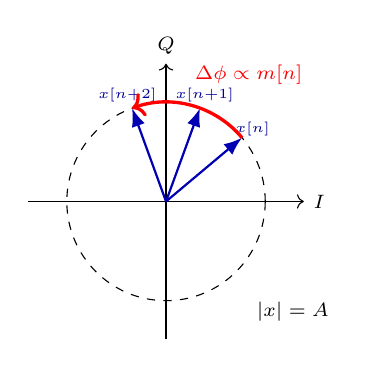
\begin{tikzpicture}[scale=0.7]
  \draw[->] (-2.5,0) -- (2.5,0) node[right] {\scriptsize $I$};
  \draw[->] (0,-2.5) -- (0,2.5) node[above] {\scriptsize $Q$};
  \draw[dashed] (0,0) circle (1.8);
  \node[font=\scriptsize] at (2.3,-2.0) {$|x|=A$};
  % Sample vectors at rotating phases
  \foreach \a/\lbl in {40/{$x[n]$},70/{$x[n{+}1]$},110/{$x[n{+}2]$}} {
    \draw[thick, blue!70!black, -{Latex}] (0,0) -- ({1.8*cos(\a)},{1.8*sin(\a)});
    \node[font=\tiny, blue!60!black]
        at ({2.05*cos(\a)},{2.05*sin(\a)}) {\lbl};
  }
  \draw[very thick, red, ->] ({1.8*cos(40)},{1.8*sin(40)}) arc (40:110:1.8);
  \node[font=\scriptsize, red] at (1.5,2.3) {$\Delta\phi \propto m[n]$};
\end{tikzpicture}
\end{center}

The rotation rate of \(x[n]\) around the origin \emph{is} the audio.
That's the whole thing.

%═══════════════════════════════════════════════════════════════════
\section{Stage 1: The DC Blocker}
%═══════════════════════════════════════════════════════════════════

\subsection{Why we need it: the direct-conversion spike}

An RTL-SDR uses a \emph{superheterodyne} architecture -- there's an
intermediate frequency (IF) stage at $\sim$\SI{3.57}{MHz}, so the
inevitable DC offsets and local-oscillator leakage in the analog chain
sit harmlessly at that IF, nowhere near baseband.  A HackRF is
\emph{direct-conversion} (zero-IF): the LO tunes exactly to \(f_c\),
mixes the signal down, and the LO leakage lands at DC in baseband --
right in the middle of your FM signal.

\begin{center}
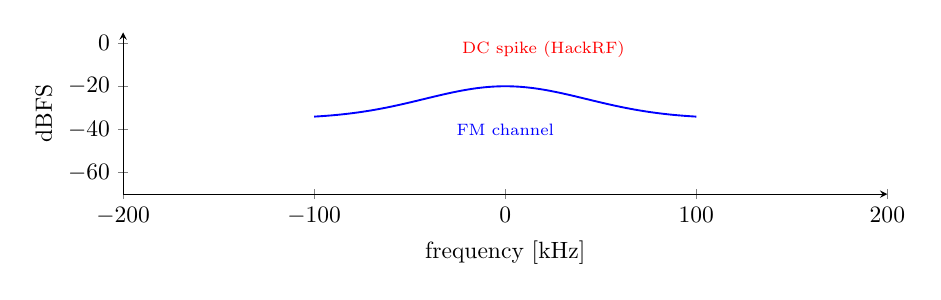
\begin{tikzpicture}[scale=0.85]
  \begin{axis}[width=13cm, height=4cm,
    ymin=-70, ymax=5,
    xlabel={frequency [\si{kHz}]}, ylabel={dBFS},
    axis y line=left, axis x line=bottom,
    xmin=-200, xmax=200, xtick={-200,-100,0,100,200}]
    % FM channel envelope
    \addplot[thick, blue, domain=-100:100, samples=200]
        {-20 - 15*(1 - exp(-((x/60)^2)))};
    % DC spike (huge)
    \addplot[very thick, red, ycomb] coordinates {(0,0)};
    \node[red, font=\scriptsize] at (axis cs:20,-3) {DC spike (HackRF)};
    \node[blue, font=\scriptsize] at (axis cs:0,-40) {FM channel};
  \end{axis}
\end{tikzpicture}
\end{center}

The FM demod that follows takes \(\angle(x[n]\,\overline{x}[n{-}1])\).
A big static DC component \(D\) turns each sample into \(x[n]+D\), so
the product becomes
\begin{equation}
(x[n]+D)\overline{(x[n{-}1]+D)}
\;=\;
x[n]\overline{x}[n{-}1] \;+\; x[n]\overline{D} \;+\; D\overline{x}[n{-}1] \;+\; |D|^2,
\end{equation}
and those cross-terms modulate the angle we're trying to read.  Result:
loud crackle, hiss, and distortion.  The fix is to kill \(D\) before
the demod.

\subsection{How we kill it: first-order IIR high-pass}

We use a simple recursive filter -- one pole, one zero -- applied
separately to \(I\) and \(Q\):
\begin{equation}
y[n] \;=\; x[n] - x[n{-}1] + R\,y[n{-}1],
\qquad R \;=\; e^{-2\pi f_c / f_s}.
\end{equation}
With \(f_c=\SI{30}{Hz}\) at \(f_s=\SI{2}{MHz}\), \(R \approx 0.99991\).
Anything below \(\sim\)\SI{30}{Hz} (including DC) is attenuated;
everything above passes through untouched.

\begin{center}
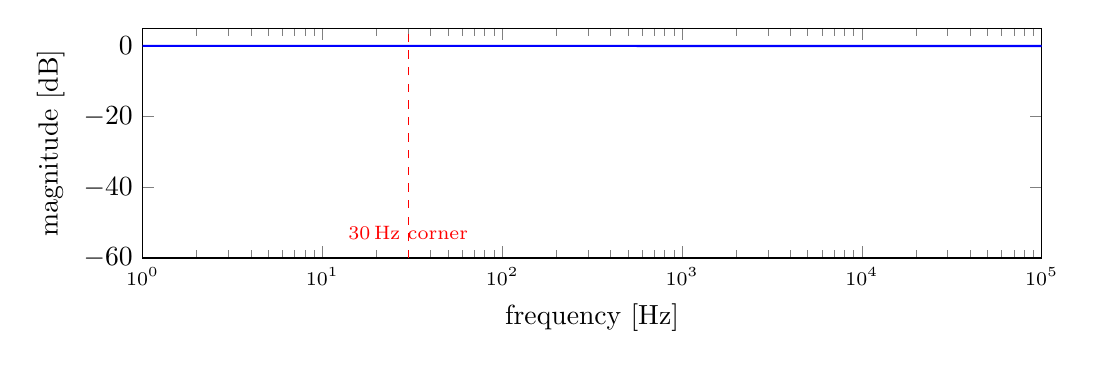
\begin{tikzpicture}
  \begin{axis}[width=13cm, height=4.5cm,
    xmode=log, ymin=-60, ymax=5,
    xlabel={frequency [\si{Hz}]}, ylabel={magnitude [dB]},
    xmin=1, xmax=100000, xtick={1,10,100,1000,10000,100000},
    xticklabel style={font=\scriptsize}]
    \addplot[thick, blue, domain=1:100000, samples=200]
      {20 * log10( sqrt(2 - 2*cos(deg(2*pi*x/2000000))) /
                   sqrt(1 - 2*0.99991*cos(deg(2*pi*x/2000000)) + 0.99991^2) )};
    \draw[dashed, red] (axis cs:30,-60) -- (axis cs:30,5);
    \node[red, font=\scriptsize] at (axis cs:30,-53) {30\,Hz corner};
  \end{axis}
\end{tikzpicture}
\end{center}

\subsection{Why not just subtract the mean?}

An earlier iteration of the code did \texttt{samples -
samples.mean()}.  That's mathematically equivalent to a very slow
moving-average high-pass, \emph{with a catch}: the DC estimate is
recomputed independently for every chunk.  If the HackRF's actual DC
offset drifts a little between chunks (thermal, gain-settling), each
chunk gets a different subtraction, leaving a small step at every
chunk boundary:

\begin{center}
\begin{tikzpicture}[scale=0.75]
  \begin{axis}[width=13cm, height=4cm,
    xlabel={time [chunks]}, ylabel={signal},
    axis y line=left, axis x line=bottom,
    xmin=0, xmax=5, xtick={0,1,2,3,4,5},
    ymin=-0.15, ymax=0.15, ytick={-0.1,0,0.1},
    title={\scriptsize per-chunk mean-subtract (bad)}]
    \addplot[thick, blue] coordinates {(0,-0.02)(1,-0.02)};
    \addplot[thick, blue] coordinates {(1,0.02)(2,0.02)};
    \addplot[thick, blue] coordinates {(2,-0.03)(3,-0.03)};
    \addplot[thick, blue] coordinates {(3,0.04)(4,0.04)};
    \addplot[thick, blue] coordinates {(4,0.01)(5,0.01)};
    % highlight the discontinuities
    \addplot[very thick, red, dashed] coordinates {(1,-0.02)(1,0.02)};
    \addplot[very thick, red, dashed] coordinates {(2,0.02)(2,-0.03)};
    \addplot[very thick, red, dashed] coordinates {(3,-0.03)(3,0.04)};
    \addplot[very thick, red, dashed] coordinates {(4,0.04)(4,0.01)};
  \end{axis}
\end{tikzpicture}
\quad
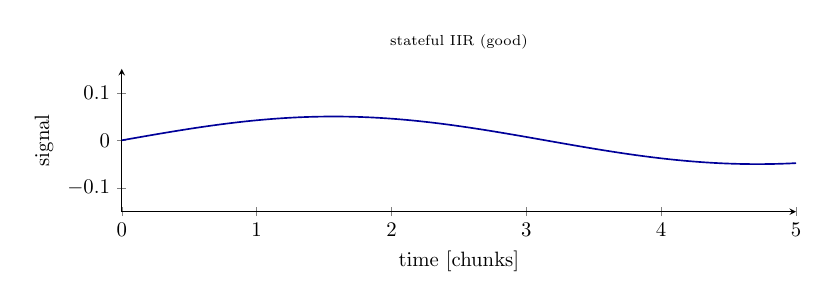
\begin{tikzpicture}[scale=0.75]
  \begin{axis}[width=13cm, height=4cm,
    xlabel={time [chunks]}, ylabel={signal},
    axis y line=left, axis x line=bottom,
    xmin=0, xmax=5, xtick={0,1,2,3,4,5},
    ymin=-0.15, ymax=0.15, ytick={-0.1,0,0.1},
    title={\scriptsize stateful IIR (good)}]
    \addplot[thick, blue!60!black, smooth, domain=0:5, samples=100]
        {0.05 * sin(deg(x))};
  \end{axis}
\end{tikzpicture}
\end{center}

At 2\,MSPS with \(2^{18}\)-sample chunks that's a step every
$\sim$130\,ms -- \(\sim\)8\,Hz -- perfectly audible as a low crackle.
The IIR carries state across chunks and doesn't have that artefact.

%═══════════════════════════════════════════════════════════════════
\section{Stage 2: The IF Channel-Select Filter}
%═══════════════════════════════════════════════════════════════════

\subsection{Why we need it}

The SDR samples the entire 2\,MHz around \(f_c\).  That's a dozen FM
channels worth of energy.  Before we can arctan-demodulate our target,
we need to throw away everything except our channel -- otherwise the
adjacent stations' spectral content contaminates the phase we're about
to read.

\subsection{Chebyshev Type-I, order 6}

We use \texttt{scipy.signal.cheby1} with 6 poles, 0.1\,dB passband
ripple, and cutoff \(w_n = \texttt{fm\_bw\_hz} / (f_s/2)\).  Chebyshev-I
gets a steep transition band for very few taps at the cost of some
passband ripple -- exactly the trade-off we want here because the
passband ripple is inaudible after the FM demod integrates it away.

\begin{center}
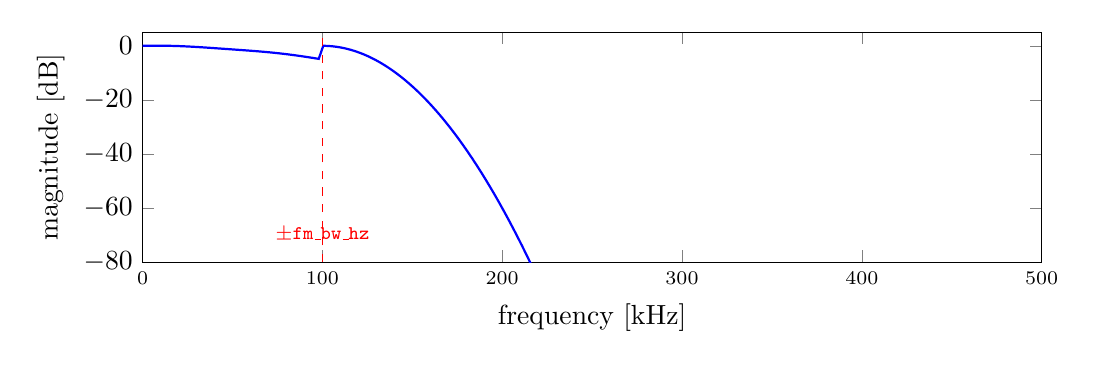
\begin{tikzpicture}
  \begin{axis}[width=13cm, height=4.5cm,
    ymin=-80, ymax=5,
    xlabel={frequency [\si{kHz}]}, ylabel={magnitude [dB]},
    xmin=0, xmax=500, xtick={0,100,200,300,400,500},
    xticklabel style={font=\scriptsize}]
    \addplot[thick, blue, domain=0:500, samples=200]
        {ifthenelse(x<100, -0.05*x*x/100 + 0.1*sin(deg(x/10)),
                            -60 * ((x-100)/100)^2)};
    \draw[dashed, red] (axis cs:100,-80) -- (axis cs:100,5);
    \node[red, font=\scriptsize] at (axis cs:100,-70) {$\pm$\texttt{fm\_bw\_hz}};
  \end{axis}
\end{tikzpicture}
\end{center}

The filter is applied to \(I\) and \(Q\) separately using
\texttt{scipy.signal.lfilter}, with state (\texttt{zi\_if\_i},
\texttt{zi\_if\_q}) preserved across chunks so no boundary artefacts.
Same trick as the DC blocker.

%═══════════════════════════════════════════════════════════════════
\section{Stage 3: FM Demodulation}
%═══════════════════════════════════════════════════════════════════

\subsection{The conjugate-product trick}

We want the audio, which equals the \emph{instantaneous frequency} of
the complex signal.  The instantaneous frequency is the time-derivative
of the phase.  In discrete time,
\begin{equation}
\omega[n] \;=\; \phi[n] - \phi[n{-}1],
\end{equation}
which we could compute as
\(\arg(x[n]) - \arg(x[n{-}1])\).  But that has an ugly modulo-\(2\pi\)
wrap-around every time the vector crosses the negative-real axis.

The slick way: multiply the current sample by the \emph{conjugate} of
the previous one.  In polar form,
\begin{equation}
x[n]\,\overline{x}[n{-}1]
\;=\; |x[n]|\,|x[n{-}1]|\,e^{\,j(\phi[n]-\phi[n{-}1])}.
\end{equation}
The phase of that product is exactly \(\phi[n]-\phi[n{-}1]\), with no
wrap-around headaches, because a single \texttt{np.angle} call
correctly handles the atan2 for a single complex number in any quadrant.

The two lines of code that do the whole demodulation:

\begin{lstlisting}[language=Python]
diff  = samples[1:] * np.conj(samples[:-1])
audio = (np.angle(diff) / np.pi).astype(np.float32)
\end{lstlisting}

We divide by \(\pi\) to normalise so that a full-scale deviation
(\(\pm\pi\) rad/sample -- physically impossible but the mathematical
maximum) maps to \(\pm 1\).  Real broadcast FM stays well within
\(\pm 0.1\) or so at 2\,MSPS.

\subsection{Geometric picture}

\begin{center}
\begin{tikzpicture}[scale=0.9]
  \draw[->] (-2.5,0) -- (2.5,0);
  \draw[->] (0,-2.5) -- (0,2.5);
  % previous sample vector
  \draw[thick, gray, -{Latex}] (0,0) -- (1.5,0) node[right, font=\scriptsize] {$x[n{-}1]$};
  % current sample vector, rotated by 30 deg
  \draw[thick, blue, -{Latex}] (0,0) -- ({1.5*cos(30)},{1.5*sin(30)})
      node[above right, font=\scriptsize] {$x[n]$};
  % arc of rotation
  \draw[thick, red, ->] (1.0,0) arc (0:30:1.0);
  \node[red, font=\scriptsize] at (1.4,0.35) {$\Delta\phi$};
  % Product vector at same angle
  \draw[dashed, thin, orange!70!black, -{Latex}] (3.5,0)
      -- ({3.5+2.0*cos(30)},{2.0*sin(30)})
      node[above right, font=\scriptsize] {$x\,\overline{x}_{-1}$};
  \draw[dashed, orange!70!black] (3.5,0) -- (5.5,0);
  \draw[dashed, orange!70!black] (4.8,0) arc (0:30:1.3);
  \node[orange!70!black, font=\scriptsize] at (5.1,0.35) {$\Delta\phi$};
\end{tikzpicture}
\end{center}

Same angle, no wrap-around, one \texttt{np.angle} call, done.

%═══════════════════════════════════════════════════════════════════
\section{Stage 4: Rational Resampling to 48\,kHz}
%═══════════════════════════════════════════════════════════════════

The demodulated audio is still at \(f_s\) (say 2\,MHz).  Our
audio-output hardware wants 48\,kHz.  \texttt{scipy.signal.resample\_poly}
does polyphase FIR resampling for any rational ratio \(L/M\).

We reduce the ratio with \texttt{gcd} first:
\begin{lstlisting}[language=Python]
g = gcd(sr, AUDIO_RATE)
self._resamp_up = AUDIO_RATE // g   # L
self._resamp_dn = sr // g           # M
\end{lstlisting}

For \(f_s=\SI{2}{MHz}\), \(f_{\text{out}}=\SI{48}{kHz}\):
\(\gcd(2000000, 48000)=2000\), so \(L=24\), \(M=1000\).  The polyphase
filter upsamples by 24 (insert zeros, then filter) and downsamples by
1000 (keep every 1000\textsuperscript{th} sample), in one efficient pass.

\begin{center}
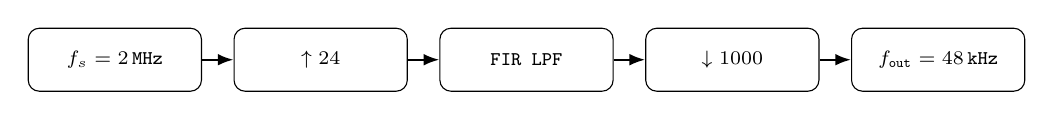
\begin{tikzpicture}[node distance=0.4cm,
  block/.style={draw, rounded corners, minimum width=2.2cm, minimum height=0.8cm,
                align=center, font=\scriptsize\ttfamily},
  arrow/.style={-{Latex[length=2mm]}, thick}]

  \node[block] (a)                {$f_s = 2$\,MHz};
  \node[block, right=of a] (b)    {$\uparrow 24$};
  \node[block, right=of b] (c)    {FIR LPF};
  \node[block, right=of c] (d)    {$\downarrow 1000$};
  \node[block, right=of d] (e)    {$f_{\text{out}} = 48$\,kHz};

  \draw[arrow] (a) -- (b);
  \draw[arrow] (b) -- (c);
  \draw[arrow] (c) -- (d);
  \draw[arrow] (d) -- (e);
\end{tikzpicture}
\end{center}

%═══════════════════════════════════════════════════════════════════
\section{Stage 5: Audio Low-Pass (15\,kHz FIR)}
%═══════════════════════════════════════════════════════════════════

After resampling we still have everything the FM demod produced up to
half the new sample rate (24\,kHz).  Broadcast FM audio bandwidth is
15\,kHz; anything above is either pilot tone leftovers, RDS, or noise.
A 64-tap FIR low-pass at 15\,kHz cleans it up:

\begin{lstlisting}[language=Python]
self._lpf_b = firwin(64, 15_000 / (AUDIO_RATE / 2)).astype(np.float32)
\end{lstlisting}

\begin{center}
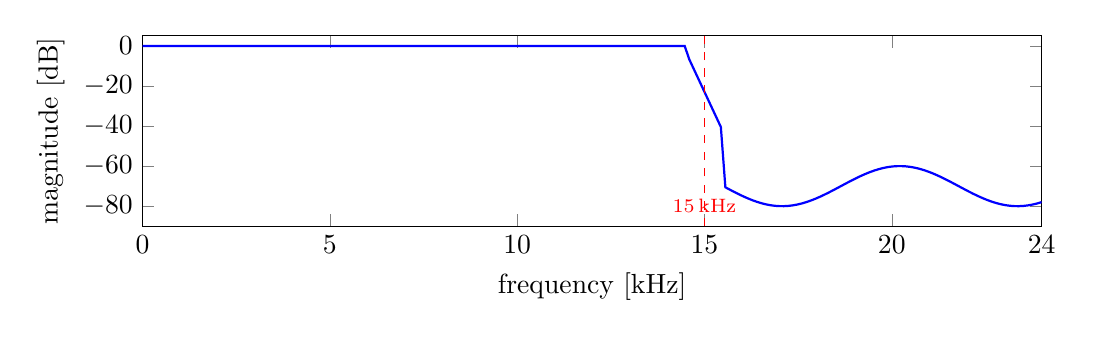
\begin{tikzpicture}
  \begin{axis}[width=13cm, height=4cm,
    ymin=-90, ymax=5,
    xlabel={frequency [\si{kHz}]}, ylabel={magnitude [dB]},
    xmin=0, xmax=24, xtick={0,5,10,15,20,24}]
    % Approximate ideal LPF shape
    \addplot[thick, blue, domain=0:24, samples=200]
        {ifthenelse(x<14.5, -0.1,
         ifthenelse(x<15.5, -3 - 40*(x-14.5),
                    -70 - 10*sin(deg(x-15.5))))};
    \draw[dashed, red] (axis cs:15,-90) -- (axis cs:15,5);
    \node[red, font=\scriptsize] at (axis cs:15,-80) {15\,kHz};
  \end{axis}
\end{tikzpicture}
\end{center}

Because it's FIR (no feedback), the state between chunks is just the
last 63 input samples -- also carried by \texttt{lfilter}'s \texttt{zi}.

%═══════════════════════════════════════════════════════════════════
\section{Stage 6: De-emphasis (50\,µs)}
%═══════════════════════════════════════════════════════════════════

\subsection{The historic reason for pre-emphasis}

FM transmitters boost the high-frequency audio content before
modulation (pre-emphasis), because FM's noise spectrum after
demodulation rises with frequency ("triangular noise").  If you didn't
compensate, high-frequency audio would sound noisy.

The receiver must apply the inverse curve -- \emph{de-emphasis} --
before you hear it, or every voice sounds like it's shouting through a
tin can.

\begin{itemize}
  \item Europe: \(\tau = \SI{50}{\micro\second}\)
  \item North America: \(\tau = \SI{75}{\micro\second}\)
\end{itemize}

\subsection{The filter}

A first-order RC low-pass with corner \(f_c = 1/(2\pi\tau)\):
50\,µs \(\Rightarrow\) 3183\,Hz.  In discrete time,
\begin{equation}
y[n] \;=\; a\,x[n] + (1-a)\,y[n{-}1],
\qquad a \;=\; \frac{\Delta t}{\tau + \Delta t},
\end{equation}
with \(\Delta t = 1/f_{\text{out}}\).  In the code:

\begin{lstlisting}[language=Python]
tau = 50e-6;  dt = 1.0 / AUDIO_RATE;  a = dt / (tau + dt)
self._de_b = np.array([a],             dtype=np.float32)
self._de_a = np.array([1., -(1. - a)], dtype=np.float32)
\end{lstlisting}

Magnitude response:

\begin{center}
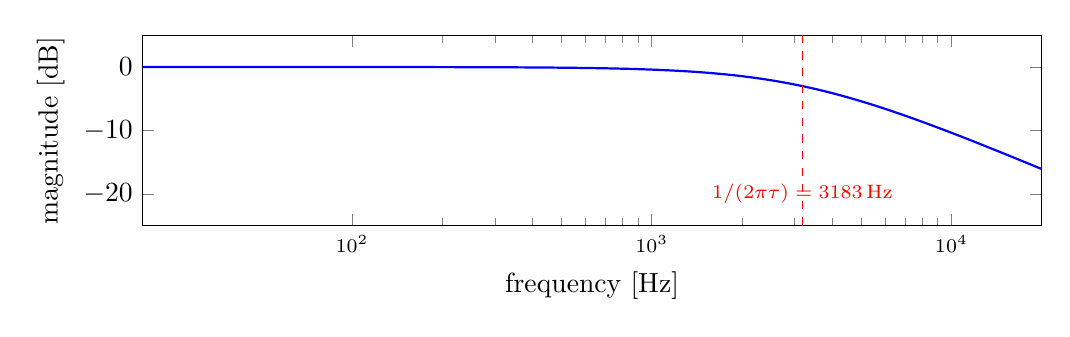
\begin{tikzpicture}
  \begin{axis}[width=13cm, height=4cm,
    ymin=-25, ymax=5,
    xlabel={frequency [\si{Hz}]}, ylabel={magnitude [dB]},
    xmode=log, xmin=20, xmax=20000,
    xtick={100,1000,10000},
    xticklabel style={font=\scriptsize}]
    \addplot[thick, blue, domain=20:20000, samples=200]
        {-10 * log10(1 + (x/3183)^2)};
    \draw[dashed, red] (axis cs:3183,-25) -- (axis cs:3183,5);
    \node[red, font=\scriptsize] at (axis cs:3183,-20) {$1/(2\pi\tau) = 3183$\,Hz};
  \end{axis}
\end{tikzpicture}
\end{center}

%═══════════════════════════════════════════════════════════════════
\section{Stage 7: Soft AGC (peak tracker)}
%═══════════════════════════════════════════════════════════════════

\subsection{The problem}

Signal strength varies a lot -- from station to station, and as
aircraft, buildings, or the operator's own hand pass the antenna.  We
don't want the OS volume slider to become the SNR knob.

\subsection{The trick}

Track a slowly-leaking peak, and normalise every chunk to it:
\begin{lstlisting}[language=Python]
peak       = float(np.max(np.abs(audio)))
self._peak = max(peak, self._peak * 0.999)
if self._peak > 1e-6:
    audio = (audio / self._peak * 0.9).astype(np.float32)
\end{lstlisting}

Each chunk, the tracker either takes the current peak (if bigger) or
decays the previous tracker value by 0.1\% (0.999\(^N\) settles over
about a second).  Divide by that tracker, scale to 0.9 to leave
headroom, done -- no clipping, no dead-quiet chunks.

\begin{center}
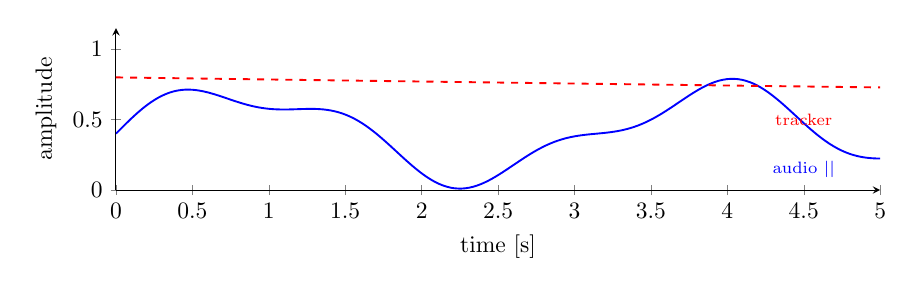
\begin{tikzpicture}[scale=0.85]
  \begin{axis}[width=13cm, height=4cm,
    xlabel={time [s]}, ylabel={amplitude},
    axis y line=left, axis x line=bottom,
    xmin=0, xmax=5, ymin=0, ymax=1.15,
    ytick={0,0.5,1}]
    % audio envelope (sinusoidal-ish variation)
    \addplot[thick, blue, domain=0:5, samples=200]
        {0.4 + 0.3 * sin(deg(2*x)) + 0.1 * sin(deg(5*x))};
    % peak tracker (envelope-follower style)
    \addplot[thick, red, dashed, domain=0:5, samples=200]
        {0.75 * exp(-0.02*x) + 0.05};
    \node[blue, font=\scriptsize] at (4.5,0.15) {audio $|·|$};
    \node[red,  font=\scriptsize] at (4.5,0.5)  {tracker};
  \end{axis}
\end{tikzpicture}
\end{center}

%═══════════════════════════════════════════════════════════════════
\section{Stage 8: Audio Output (ring buffer + PortAudio)}
%═══════════════════════════════════════════════════════════════════

The final stage isn't DSP, it's plumbing.  \texttt{sounddevice} (a
PortAudio wrapper) opens an output stream at \SI{48}{kHz}, one channel,
32-bit float, and calls our \texttt{\_audio\_callback} whenever the
soundcard needs more samples.  The demodulator's \texttt{process()} and
the audio callback share a single \texttt{numpy} buffer through a lock:

\begin{center}
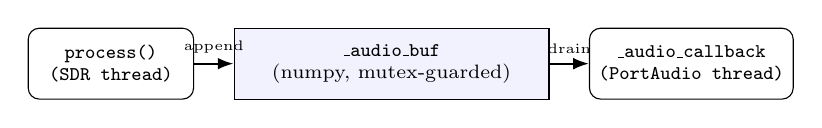
\begin{tikzpicture}[node distance=0.5cm,
  block/.style={draw, rounded corners, minimum width=2.1cm, minimum height=0.9cm,
                align=center, font=\scriptsize\ttfamily},
  buf/.style={draw, fill=blue!5, minimum width=4cm, minimum height=0.9cm,
              align=center, font=\scriptsize},
  arrow/.style={-{Latex[length=2mm]}, thick}]

  \node[block]                                (p) {\texttt{process()}\\(SDR thread)};
  \node[buf, right=of p]                      (b) {\texttt{\_audio\_buf}\\(numpy, mutex-guarded)};
  \node[block, right=of b]                    (c) {\texttt{\_audio\_callback}\\(PortAudio thread)};
  \draw[arrow] (p) -- node[above, font=\tiny] {append} (b);
  \draw[arrow] (b) -- node[above, font=\tiny] {drain}  (c);
\end{tikzpicture}
\end{center}

The buffer is capped at 2\,s of audio (\SI{96000}{samples}) so that if
the SDR side gets ahead of playback we drop older audio rather than
letting latency grow unboundedly.

%═══════════════════════════════════════════════════════════════════
\section{Summary Table}
%═══════════════════════════════════════════════════════════════════

\begin{center}
\begin{tabular}{@{}rlll@{}}
\toprule
\textbf{Stage} & \textbf{Purpose} & \textbf{Filter}   & \textbf{Cost per chunk} \\
\midrule
1 & DC block         & IIR HP, $f_c{\approx}30$\,Hz          & 2 real \texttt{lfilter}s \\
2 & Channel select   & Chebyshev-I 6-pole LPF                & 2 real \texttt{lfilter}s \\
3 & FM demod         & $\arg(x\,\overline{x}_{-1})$          & 1 complex mul + \texttt{np.angle} \\
4 & Resample $\to$ 48\,kHz & Polyphase FIR ($L{=}24$, $M{=}1000$) & 1 \texttt{resample\_poly} \\
5 & Audio LPF        & 64-tap FIR, $f_c{=}15$\,kHz           & 1 real \texttt{lfilter} \\
6 & De-emphasis      & 1-pole IIR, $\tau{=}50\,\mu$s         & 1 real \texttt{lfilter} \\
7 & Soft AGC         & Peak envelope tracker                 & 1 \texttt{max} + broadcast div \\
8 & Audio out        & Ring buffer $\to$ PortAudio           & memcpy \\
\bottomrule
\end{tabular}
\end{center}

Total cost is dominated by stages 2 and 4.  On a Raspberry Pi 4 at
\SI{2}{MSPS} the whole pipeline runs at $\sim$5\% of one core --
plenty of headroom for the RDS decoder, spectrum, and the record
plugin to run in parallel.

%═══════════════════════════════════════════════════════════════════
\section{Things We Deliberately Don't Do}
%═══════════════════════════════════════════════════════════════════

\begin{itemize}
  \item \textbf{Stereo decode.}  We ignore the 19\,kHz pilot and the
        L$-$R DSB-SC.  Adding stereo means a PLL locked to the pilot
        and a synchronous demodulator around 38\,kHz; nontrivial but
        not hard.  Filed under future additions if anyone actually
        wants it.
  \item \textbf{LO offset tuning.}  We tune \(f_c\) directly at the
        station carrier, then rely on the DC blocker to swallow the
        centre spike.  Sidestep is arguably nicer: tune 200--500\,kHz
        \emph{off} the station and NCO-mix the target down to DC in
        software.  Never sees the spike at all.  Bigger change (needs
        an offset in the \texttt{AppState}, a complex mixer in the
        plugin) -- listed in \texttt{ideas.md}.
  \item \textbf{Automatic squelch.}  Very handy for scanning, but our
        FM plugin is stateless per-station: tune, listen, retune.
        Squelch would need a running SNR estimate we don't currently
        maintain.
\end{itemize}

%═══════════════════════════════════════════════════════════════════
\section{Bibliography and Further Reading}
%═══════════════════════════════════════════════════════════════════

\begin{itemize}
  \item Lyons, R.\ G., \emph{Understanding Digital Signal Processing},
        3rd ed.  Ch.\ 13 (analytic signals and phase-derivative
        demodulation) and Ch.\ 10 (multirate).
  \item Rice, M., \emph{Digital Communications: A Discrete-Time
        Approach}.  Ch.\ 5 on FM and phase-locked loops.
  \item ITU-R BS.450-3, \emph{Transmission standards for FM sound
        broadcasting at VHF} -- the pre-emphasis time constants,
        stereo MPX layout, RDS placement, etc.
  \item scipy.signal documentation on \texttt{lfilter},
        \texttt{cheby1}, \texttt{firwin}, and \texttt{resample\_poly}.
\end{itemize}

\end{document}
